

%%%%%%%%%%%%%%%%%%%%%%%%%%%%%%%%%%%%%%%%%%%%%%%%%%%%
\subsection{NWChem Quantum Chemistry Application}\label{sec:eva-realapp}
%%%%%%%%%%%%%%%%%%%%%%%%%%%%%%%%%%%%%%%%%%%%%%%%%%%%

NWChem~\cite{NWChem63} is a computational chemistry application suite
offering many simulation capabilities.  For massively
parallel simulations, a common method employed is coupled-cluster
theory (CC), for which NWChem has extensive
functionality~\cite{Hirata:2003:JPCA:TCE} and excellent
performance~\cite{Apra:2009:SC:NWChem}.  For data movement, NWChem uses the Global
Arrays~\cite{GA_SC94} toolkit, which has been
implemented on a number of platforms natively and as a portable
implementation over MPI RMA~\cite{dinan12:armci_mpi}.

Because CC simulations are one of the most common usages of NWChem in
the context of large clusters or supercomputers, our experiments focus
on the most popular CC method, CCSD(T).
Two molecules are considered: the water cluster (H$_2$O)$_n$
($n=16$)---denoted W$n$ for short---and C$_{20}$, obtained
from the NWChem QA test suite (\texttt{QA/tests/tce\_c20\_triplet}).
For the water cluster, we used double-zeta basis sets (cc-pVDZ from
the NWChem basis set library), which are reasonable for this class of
problems.  We compared Casper with both the original MPI and two
thread-based approaches.
The first approach employs oversubscribed cores
(Thread~(O)), where every thread and its MPI process execute on
the same core; the second approach uses dedicated cores (Thread~(D)),
where threads and MPI processes are on separate cores. We used the same total
number of cores in all approaches, some of which are dedicated to
asynchronous ghost processes\slash threads as listed in Table~\ref{tab:eva-nwcore}.

\begin{table}\scriptsize
\begin{center}
\caption{Core deployment in NWChem evaluation on Cray XC30.}\label{tab:eva-nwcore}
\begin{tabular}{|c|c|c|}
\hline
& Computing Cores & Async Cores \\
\hline
Original MPI & 24 & 0 \\
Casper & 20 & 4 \\
Thread (O) & 24 & 24 \\
Thread (D) & 12 & 12 \\
\hline
\end{tabular}
\end{center}
% \vspace{-4.0ex}
\end{table}

Figures~\ref{fig:eva-edison-nw-w16} and
\ref{fig:eva-edison-nw-c20-ccsd} report timings for a single
iteration of CCSD, which is a communication-intensive solver composed
of more than a dozen tensor contractions of varying size.  For smaller
problems, when computation dominates, asynchronous progress is more
important because the application is calling MPI relatively
infrequently.  At larger scale, the computation time decreases, and the
communication is more frequent; hence the improvement with Casper is
less.  The (T) portion of the CCSD(T) methods is much more
compute-intensive. Hence, the time between MPI calls can be
large, and thus the impact of asynchronous progress is
significant.  Each process fetches remote data, then does significant
computation---over and over. As a result, the lack of progress causes
processes to stall, waiting on GET operations to be satisfied remotely.
Figure~\ref{fig:eva-edison-nw-c20-ccsdt} shows the significance of
asynchronous progress at all scales.  Relative to the original
version, Casper is almost twice as fast; but thread-based asynchronous
progress is far less effective. The reason is that although both approaches
improve asynchronous progress in communication, the thread-based
solutions significantly degrade the performance of computation, either by
core oversubscription or by appropriation of half of the computing cores.

\begin{figure*}
\centering
\subfigure[CCSD for W16=(H$_2$O)$_{16}$ with pVDZ]{
  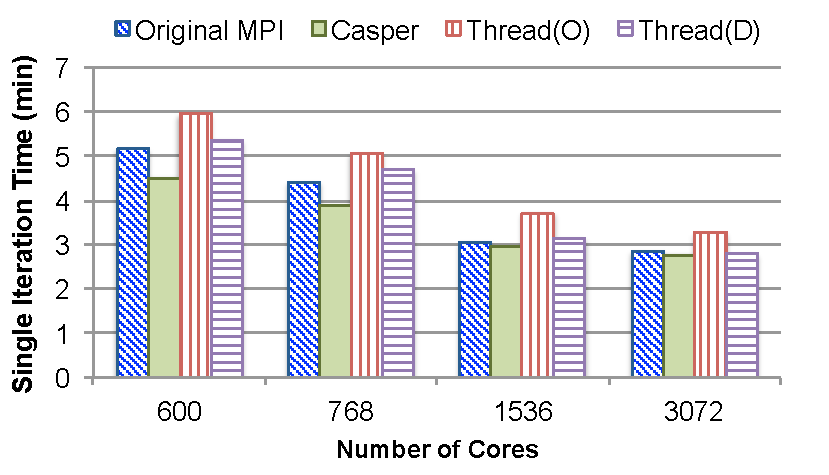
\includegraphics[width=0.64\columnwidth]{figures/casper/eva_edison_nwchem_w16_dz.pdf}
  \label{fig:eva-edison-nw-w16}
}
\subfigure[CCSD for C$_{20}$ with pVTZ]{
  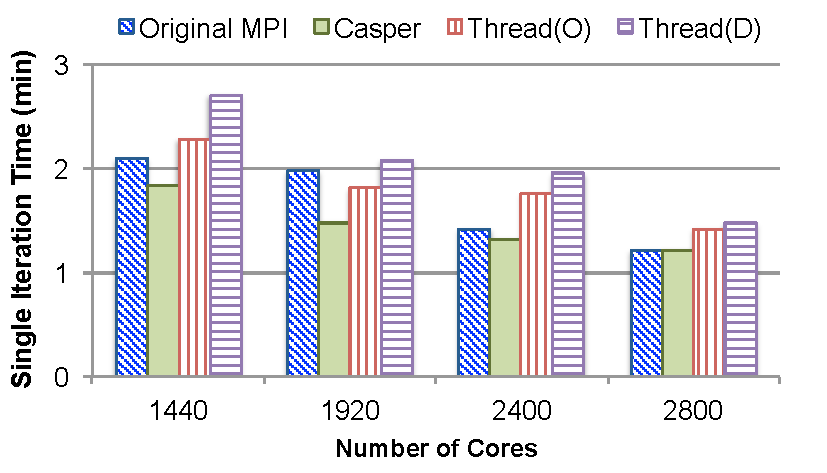
\includegraphics[width=0.64\columnwidth]{figures/casper/eva_edison_nwchem_tce_c20_ccsd.pdf}
  \label{fig:eva-edison-nw-c20-ccsd}
}
\subfigure[(T) portion of CCSD(T) for C$_{20}$ with pVTZ]{
  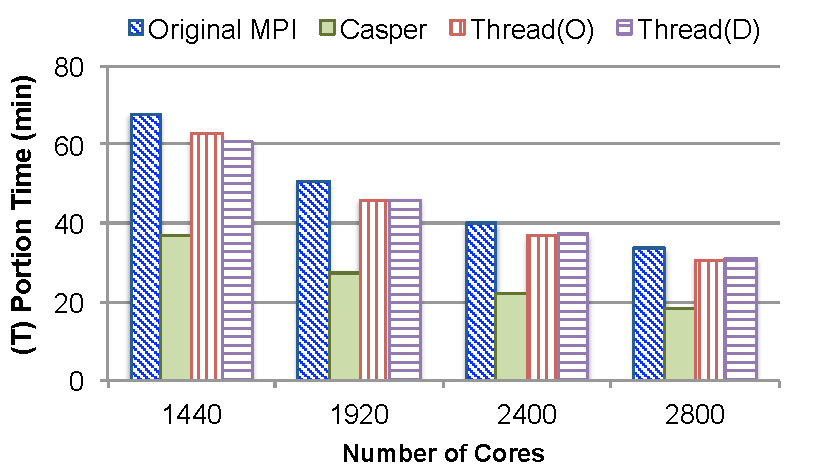
\includegraphics[width=0.64\columnwidth]{figures/casper/eva_edison_nwchem_tce_c20_ccsdt.pdf}
  \label{fig:eva-edison-nw-c20-ccsdt}
}
% \vspace{-1.0ex}
\caption{NWChem TCE coupled cluster methods on Cray XC30.}
\label{fig:eva-nwchem}
% \vspace{-4.0ex}
\end{figure*}

